\chapter{无人机编队整体控制逻辑、仿真环境以及硬件选型}
\label{chap:hardware}
本章主要介绍无人机编队的编队控制算法之外的系统组成部分;之后介绍无人机编队的整体的控制的实现逻辑,之后将介绍无人机编队的动力学仿真环境的搭建。
最后将介绍本次设计之中所用到的无人机型号,自动驾驶仪硬件以及姿态自动驾驶仪内环基本控制逻辑。
\section{ 软件控制逻辑以及软件环境 }
编队控制算法所运行的软件环境是ROS(Robot Operating System)。ROS是一个适用于机器人的开源操作系统。
它提供了操作系统应有的服务,包括硬件抽象,底层设备控制,常用函数实现,进程间消息传递,以及包管理。
它也提供用于获取、编译、编写、和跨计算机运行代码所需的工具和库函数。本次使用的应用程序接口是ROS下的mavros功能包,
本功能包的作用是:将来自自动驾驶仪的无人机状态数据由mavlink通信协议转换为ROS的进程间的通讯的协议;
将来自编队控制器的姿态驾驶仪内环的期望姿态角以及期望油门值按照mavlink的协议进行编码,从而起到沟通编队控制器以及姿态驾驶仪内环的桥梁作用。

自动驾驶仪则使用第\ref{chap:single_control_logic}章中介绍的PX4开源自驾仪,此处不再赘述。
\section{无人机软硬件环境选配}
本文所设计的编队控制器是以开源自动驾驶仪PX4的内环为基础的,PX4的内环自动驾驶仪运行在Pixhawk这一开源硬件之上,成为上层控制的下位机(slave computer):
编队控制算法运行在具有ROS环境的上位机(host computer)中;
整体的软件硬件选配关系如下图所示:
\begin{figure}[H]
    \centering
    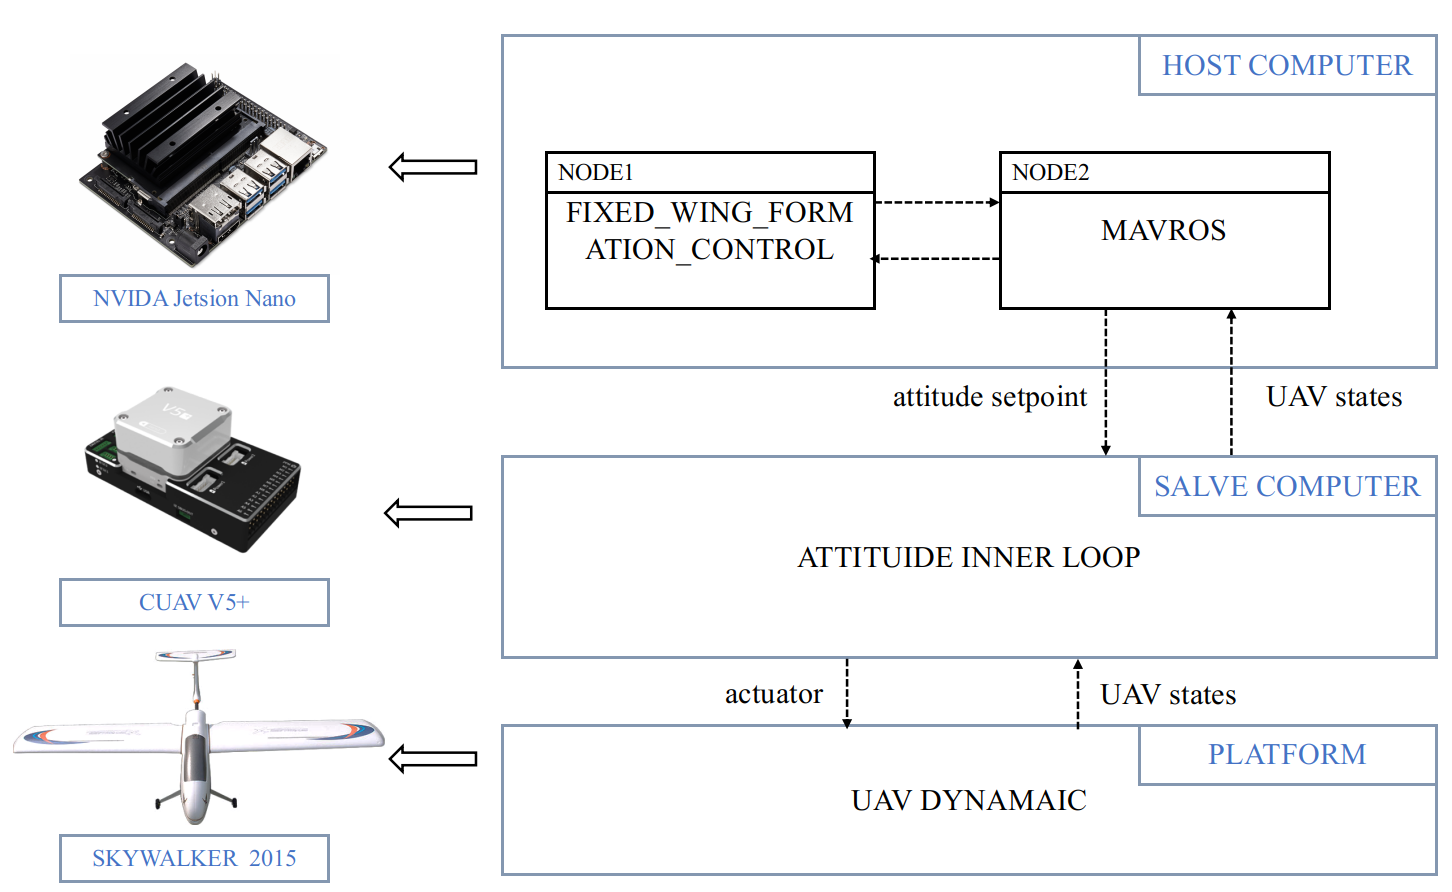
\includegraphics[width=1\textwidth]{figures/c4/c4-soft-hard.png}
    \caption{硬件软件选配关系}\label{fig:c4-soft-hard.png}
\end{figure}
上位机(host computer)的选择主要由其性能决定,应满足ROS基本环境的正常运行以及编队控制算法的需求;其次应考虑该硬件的寿命,体积,工况
要求等指标。下位机(slave computer)是PX4等算法运行的介质,也是飞行之中的重要传感器如惯性原件(IMU)、磁罗盘以及定位模块(GPS Module)的
工作平台,选择时考虑其传感器精度,平台计算能力等因素;无人机是编队控制的载具平台,应根据上述硬件以及必要航电设备选择翼面积、起飞质量
有效载荷等重要参数;根据硬件安放位置选择合适的机舱外形;根据编队控制需要确定平飞速度;根据期望推力选择发动机型号;根据起飞降落方式
选择起落架类型。必要时,应根据性能要求以及指标设计无人机。

在无人机编队过程中,双机通信必不可少。通信模块相对于无人机系统相对独立,在此只介绍硬件实现的一种手段:通讯模块选用P900芯片,通讯协议
选用mavlink协议,驱动由ROS下的串口功能包“serial”提供;实际双机编队飞行试验的硬件链接逻辑如下图所示:


\section{无人机编队动力学仿真环境}
所谓无人机动力学仿真环境,是在考虑无人机的动力学过程的基础之上搭建的仿真环境,相较于控制器的数学仿真,此种仿真环境考
虑了无人机作为一个实际的被控系统而存在的过渡过程,不确定性以及扰动因素,将更加符合无人机飞行时的实际状态。
本次动力学仿真环境基于Gazebo这一通用的开源仿真环境仿真环境,除调用物理引擎仿真飞行器6自由度的动力学模型外,还可以产生相应的、添加噪声
污染的传感器数据反馈给下位机自动驾驶仪。
\begin{figure}[H]
    \centering
    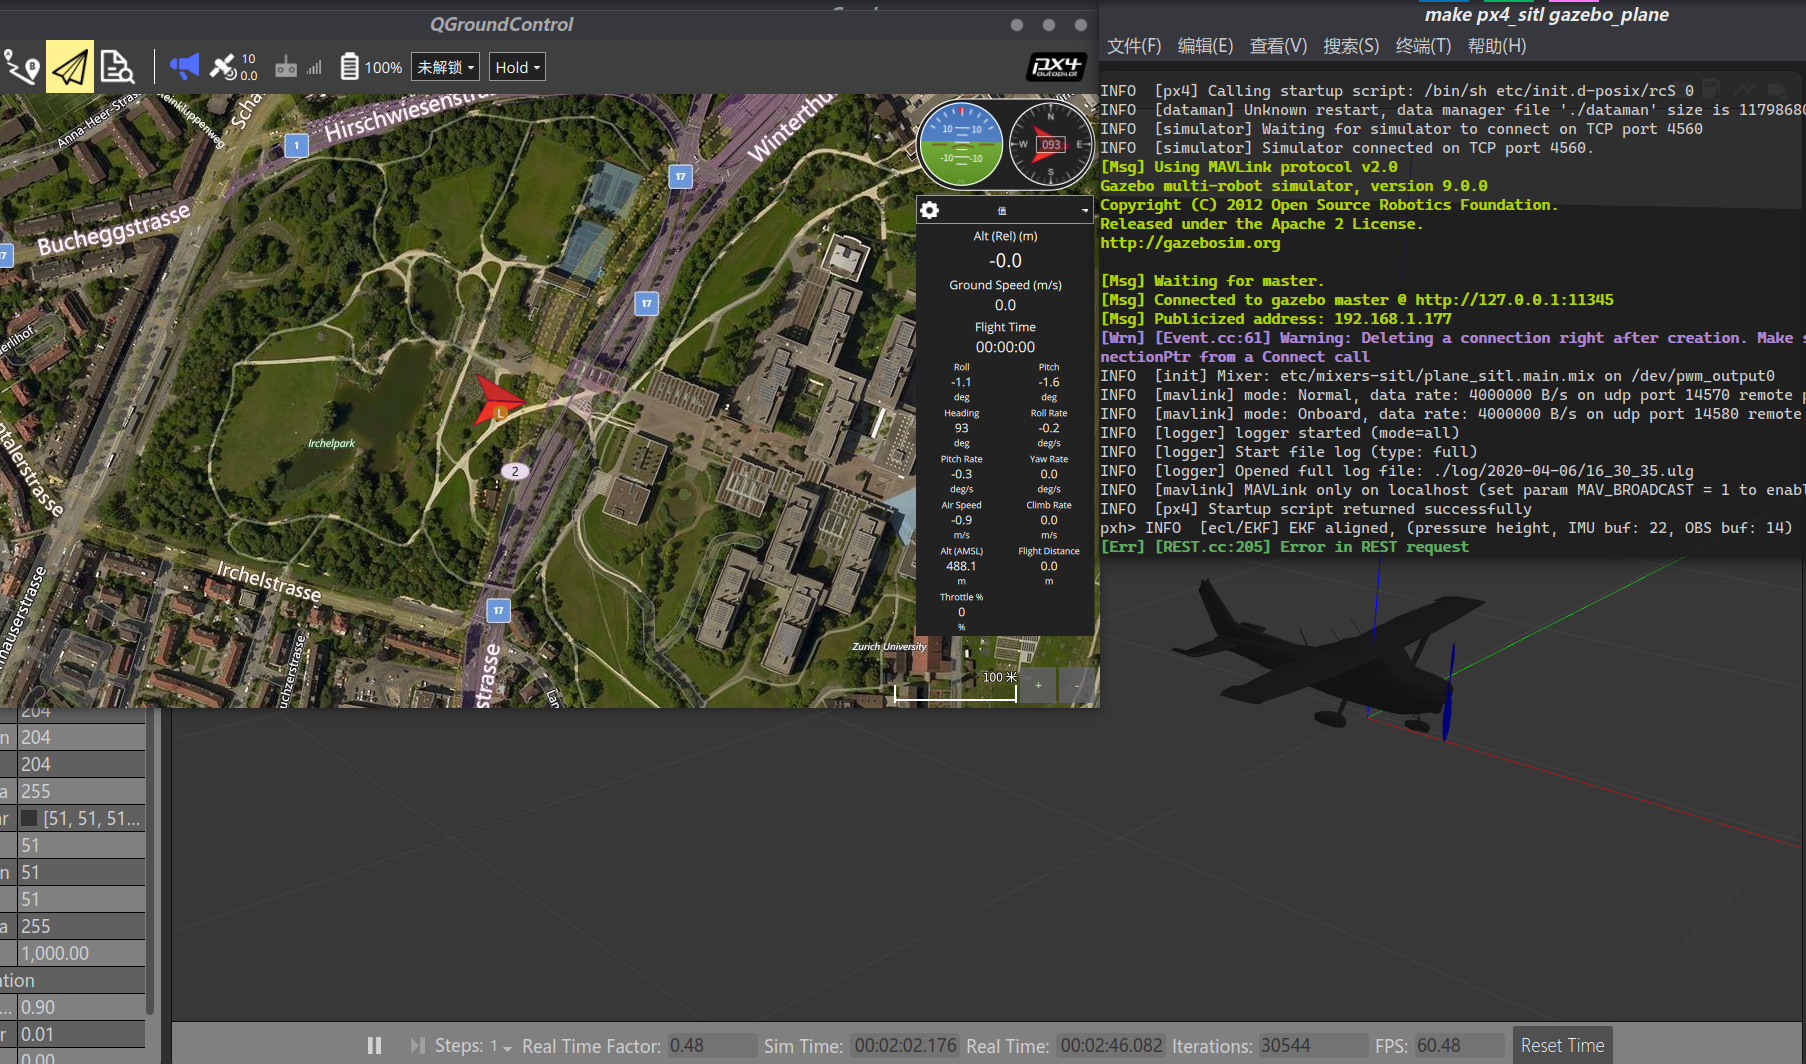
\includegraphics[width=0.75\textwidth]{figures/c4/Gazebo.png}
    \caption{Gazebo仿真环境}\label{fig:c4-Gazebo}
\end{figure}

仿真之中的飞机的动力学模型由Gazebo仿真环境给出,可自定义飞机的质量,推力等参数;仿真之中的传感器数据由Gazebo产生,由PX4读取,作为
真实环境之中的传感器数据的仿真。基于ROS的编队控制程序同时运行,通过mavros等程序API进行数据交互,完成动力学仿真。
相应的仿真程序之间的逻辑关系如下图所示:
\begin{figure}[H]
    \centering
    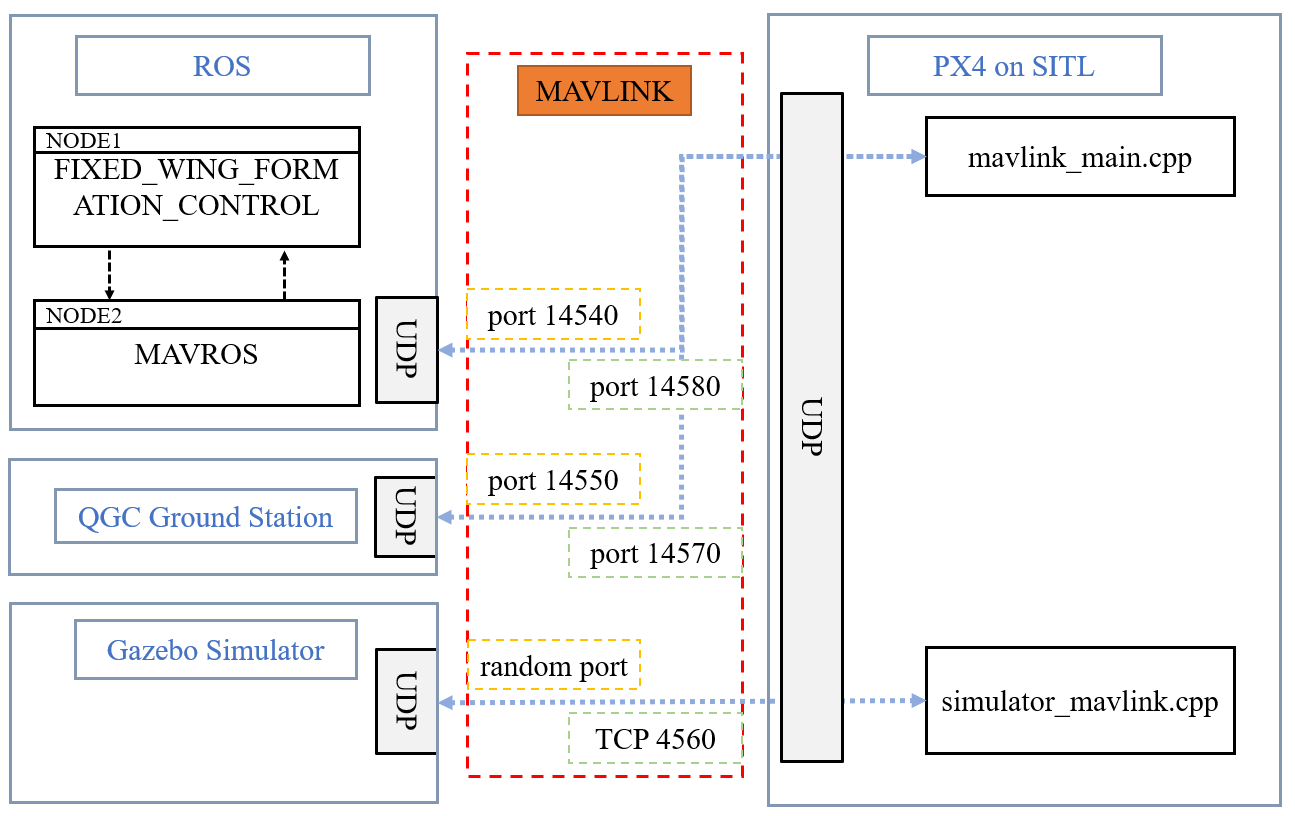
\includegraphics[width=0.75\textwidth]{figures/c4/px4_sitl_overview.png}
    \caption{编队控制仿真逻辑}\label{fig:px4_sitl_overview}
\end{figure}
